\subsection{Post-trained Model Evaluations}
\label{subsec:final_model_evals}
\subsubsection{Evaluation Setup}

We evaluate \ourmodel on a comprehensive suite of benchmarks spanning agentic capabilities, reasoning and knowledge, conversational ability and instruction following, long-context understanding, and multilingual performance.
All evaluation results for \ourmodel and baselines were collected via Nemo Evaluator SDK\footnote{\url{https://github.com/NVIDIA-NeMo/Evaluator}}. We used three main evaluation harnesses: Nemo Gym\footnote{\url{https://github.com/NVIDIA-NeMo/Gym}}, Nemo Skills\footnote{\url{https://github.com/NVIDIA-NeMo/Skills}}, and Harbor\footnote{\url{https://github.com/harbor-framework/harbor}} with extended sandboxing support via AWS ECS on Nemo Evaluator. In addition, the evaluations also used dedicated open-source packaged containers for Multi-Challenge Multi-Turn Instruction Following. For reproducibility purposes, more details on the evaluation settings and pinned containers can be found in the Nemo Evaluator SDK examples folder\footnote{\url{https://github.com/NVIDIA-NeMo/Evaluator/blob/main/examples/nemotron/nemotron-3-ultra}} and the corresponding reproducibility tutorial.

The following benchmarks are not onboarded yet in our open source tools and for these we used either their official open source implementation or otherwise an internal scaffolding that we plan to open source in the future: BrowseComp, Tau Bench 3, ProfBench, PinchBench, Vals.ai Financial Agent, LongBench v2.

All models were evaluated under the same evaluation settings including agentic resources (CPU compute and timeouts), input data, prompt templates, number of repeats, and extraction/metric implementation. Inference parameters such as temperature and top\_p, and maximum number of tokens were directly extracted from the recommendations of the corresponding model cards. 

\paragraph{Agentic Capabilities.}
We evaluate agentic capabilities using Terminal-Bench 2.1~\citep{merrill2026terminal} for terminal-based task execution; GDPVal~\citep{patwardhan2025gdpval} for economically valuable real-world workplace tasks; SWE-Bench Verified~\citep{jimenez2023swe} and SWE-Bench Multilingual~\citep{jimenez2023swe} for software engineering agents; ProfBench~\citep{wang2026profbench} for professional-domain reasoning and deep-research tasks; PinchBench~\citep{pinchbench_skill2026} for coding agents in OpenClaw environments; TauBench V3~\citep{barres2025tau} for conversational tool use; BrowseComp~\citep{wei2025browsecomp} for web browsing and information-seeking tasks; and the Vals.ai Financial Agent Benchmark~\citep{bigeard2025finance} for financial analysis and decision-support tasks.

\paragraph{Reasoning and Knowledge.}
We evaluate reasoning and knowledge capabilities across coding, mathematics, scientific reasoning, and expert-level knowledge domains. For coding and algorithmic problem solving, we use International Olympiad in Informatics (IOI) 2025~\citep{ioi2025} and LiveCodeBench v6~\citep{jain2024livecodebench}. Mathematical reasoning is assessed using IMO-AnswerBench~\citep{luong2025towards} and MathArena Apex-Shortlist~\citep{dekoninck2026matharena}. For IMO-AnswerBench and Apex-Shortlist, we report both \emph{without-tools} and \emph{with-tools} settings, where the latter allows the model to use Python for computation and verification during problem solving. We further evaluate expert-level knowledge and reasoning using GPQA~\citep{rein2023gpqa}, MMLU-Pro~\citep{wang2024mmlupro}, and Humanity's Last Exam (HLE)~\citep{phan2025humanitysexam}; scientific coding with SciCode~\citep{tian2024scicoderesearchcodingbenchmark}; research-level physics reasoning with CritPt~\citep{zhu2025critpt}; and factual reliability and hallucination resistance with AA-Omniscience~\citep{jackson2025aaomniscience}. Together, these benchmarks provide a comprehensive assessment of the model's reasoning, problem-solving, and knowledge capabilities across a wide range of domains.


\paragraph{Conversation and Instruction Following.}
We assess conversational quality and instruction-following ability using IFBench~\citep{pyatkin2025generalizing}, and Multi-Challenge~\citep{deshpande2025multichallenge}. IFBench measures instruction-following accuracy under verifiable constraints. Multi-Challenge evaluates multi-turn conversational competence.

\paragraph{Long-Context Understanding.}
We evaluate long-context capabilities using AA-LCR~\citep{artificialanalysis2025lcr}, RULER~\citep{hsieh2024ruler}, and LongBench v2~\citep{bai2025longbenchv2}, which measure information retrieval, synthesis, and reasoning over long contexts of up to one million tokens.

\paragraph{Multilingual Performance.}
We evaluate multilingual capabilities using MMLU-ProX~\citep{xuan2025mmluprox} and WMT24++~\citep{deutsch2025wmt24pp} for multilingual reasoning, knowledge, and machine translation.

For more details, please refer to Appendix \ref{appendix:eval}.


\subsubsection{Evaluation Results}

% \begin{table*}[!t]
% \centering
% \footnotesize
% \setlength{\tabcolsep}{2.5pt}
% \renewcommand{\arraystretch}{1.05}

% \resizebox{\textwidth}{!}{%
% \begin{tabular}{l|c c c c c c c}
% \toprule
% \textbf{Benchmark}
% & \makecell{\textbf{N-3-Ultra}\\\textbf{550B-A55B}}
% & \makecell{\textbf{GLM-5.1}\\\textbf{744B-A40B}}
% & \makecell{\textbf{MiniMax-2.7}\\\textbf{230B-A10B}}
% & \makecell{\textbf{Kimi-K2.6}\\\textbf{1T-A32B}}
% & \makecell{\textbf{Qwen-3.5}\\\textbf{397B-17B}}
% & \makecell{\textbf{DS-v4-Pro}\\\textbf{1.6T-A49B}}
% & \makecell{\textbf{DS-v4-Flash}\\\textbf{284B-A13B}} \\
% \midrule
% \rowcolor{black!5}
% \multicolumn{8}{l}{\textbf{Agentic}} \\
% \midrule
% Terminal Bench 2.1 & 56.4 & 59.3 & 55.5 & 67.2 & 49.9 & 49.2 & 54.2 \\
% GDPVal & 46.7 & 54.7 & 47.6 & 50.4 & 34.6 & 54.6 & 50.2\\
% SWE-Bench Verified & 71.9 & 73.8 &	72.2 &	69.5 &	69.9 &	74.0 &	72.4 \\
% SWE-Bench Multilingual & 67.7 & 73.8 &	69.2 &	65.9 &	67.7 &	71.9 &	72.1 \\
% ProfBench (Search) & 56.0 & 46.0 & 52.0 & 56.0 & 53.0 & 59.9 & 57.0 \\
% PinchBench & 90.0 & 81.2 & 77.6 & 90.2 & 86.6 & 88.6 & 91.3 \\
% TauBench V3 & & & & & & \\
% \quad Airline & 81.5& 85.0& 75.3 & 85.8& 76.5 & 80.8 & 80.8\\
% \quad Retail & 86.4& 84.1& 84.9 & 82.9& 88.5 & 88.9 & 89.1 \\
% \quad Telecom & 92.9& 96.9& 89.6 & 97.8 & 98.0& 96.3 & 98.3\\
% \quad Banking & 22.6 & 12.8 & 14.6 & 23.1 & 20.9 & 25.9 & 26.7 \\
% \quad Average & 70.9 & 69.7 & 66.1 & 72.4 & 71.0 & 73.2 & 73.7 \\
% BrowseComp & 44.4  & 59.4 & 54.1 & 61.3 & 40.5 & 59.4 & 46.9  \\
% Vals.ai Financial Agent 1.1 & & & & & & \\
% \quad without web search & 60.1 & 60.2 & 51.3 & 54.0 & 61.3 & 58.9 & 58.4\\
% \quad with web search & 53.7 & 60.7 & 50.5 & 58.8 & 59.0 & 62.3 & 60.1\\

% \midrule
% \rowcolor{black!5}
% \multicolumn{8}{l}{\textbf{Reasoning and Knowledge}} \\
% \midrule
% IOI 2025 & 570.0 & 456.5 & -- & 585.0 & 441.3 & 580.1 & --\\
% LiveCodeBench (v6) & 89.0& 85.7 & 77.2 & 90.2 & 79.3 & 92.5 & 90.9 \\
% IMOAnswerBench (no tools) & 88.6& 86.8 & 68.3 & 91.1 & 83.1 & 93.0 & 91.1 \\
% IMOAnswerBench (with tools) & 92.3 & 91.1 & 75.1 & 93.71 & 84.51 & 85.4 & 89.6 \\
% % IMOAnswerBench (with tools) & 91.4 & 91.1 & 75.1 & 93.7 & 84.5 & 85.4 & 89.6 \\
% Apex-Shortlist (no tools) & 74.9 & 71.1 & 28.9 & 77.4 & 61.4 & 85.8 & 82.4 \\
% Apex-Shortlist (with tools) & 84.8 & 79.0 & 51.9 & 73.2 & 60.4 & 86.5 & 82.0 \\
% % IMOProofBench & & & & & & \\
% GPQA (no tools) & 87.0 & 86.1 & 86.6 & 91.0 & 87.1 & 87.8 & 88.5 \\
% SciCode (subtask) & 44.6 & 47.7 & 38.3 & 52.0 & 48.0 & 50.5 & 48.2 \\
% HLE (no tools) & 26.7 & 27.2 & 23.1 & 34.8 & 28.5 & 37.7 & 32.2 \\
% HLE (with tools) & 37.4 & 50.4 & --  & 54.0 & 48.3 & 48.2 & 45.1 \\
% CritPt (no tools) & 3.1 & 3.7 & 0.6 & 9.1 & 2.4 & 14.0 & 10.6\\
% % CritPt (with tools) & & & & & & \\
% MMLU-Pro & 86.8 & 85.9 & 81.9 & 88.1 & 88.3 & 87.5 & 86.4\\
% OmniScience Accuracy & 24.1 & 31.3 & 20.5 & 35.5 & 35.9 & 46.8 & 39.9\\
% OmniScience Non-Hallucination & 78.7 & 66.8 & 74.4 & 67.1 & 7.4 & 5.7 & 2.8\\

% \midrule
% \rowcolor{black!5}
% \multicolumn{8}{l}{\textbf{Chat \& Instruction Following}} \\
% \midrule
% IFBench (prompt loose) & 81.7 & 76.6 & 74.6 & 73.7 & 78.2 & 79.1 & 82.0 \\
% Multi-Challenge & 63.8 & 63.0 & 42.5 & 63.1 & 63.9 & 64.1 & 63.5\\
% Arena-Hard-V2 & 88.1 & 78.7 & 66.0 & 85.6 & 81.5 & 78.1 & 77.0 \\

% \midrule
% \rowcolor{black!5}
% \multicolumn{8}{l}{\textbf{Long Context}} \\
% \midrule
% AA-LCR & 65.4 & 66.9 & 69.8 & 70.2 & 68.3 & 67.3 & 62.7 \\
% RULER (1M) & 94.7 & -- & -- & -- & 90.1 & 94.2 & 87.7 \\
% Longbench v2 ($\leq$ 1M) & 61.9 & -- & -- & -- & 68.9 & 62.1 & 57.0 \\
% \midrule
% \rowcolor{black!5}
% \multicolumn{8}{l}{\textbf{Multilingual}} \\
% \midrule
% MMLU-ProX (avg en/de/fr/es/it/ja/zh/hi/pt/ko) & 83.0 & 85.8 & 78.4 & 85.0 & 86.4 & 85.6 & 84.3\\
% WMT24++ (en$\rightarrow$xx) & 83.7 & 84.4 & 82.8 & 84.5 & 86.8 & 85.9 & 85.9 \\

% \bottomrule
% \end{tabular}%
% }

% \caption{
% Evaluation suite for \ourmodel. We compare against six open models.
% }
% \label{tab:ultra_comparison}
% \end{table*}


\begin{table*}[!t]
\centering
\footnotesize
\setlength{\tabcolsep}{2.5pt}
\renewcommand{\arraystretch}{1.05}

\resizebox{\textwidth}{!}{%
\begin{tabular}{l|c c c c c c c}
\toprule
\textbf{Benchmark}
& \makecell{\textbf{N-3-Ultra}\\\textbf{550B-A55B}}
& \makecell{\textbf{MiniMax-2.7}\\\textbf{230B-A10B}}
& \makecell{\textbf{GLM-5.1}\\\textbf{744B-A40B}}
& \makecell{\textbf{Kimi-K2.6}\\\textbf{1T-A32B}}
& \makecell{\textbf{Qwen-3.5}\\\textbf{397B-17B}}
& \makecell{\textbf{DS-v4-Pro}\\\textbf{1.6T-A49B}}
& \makecell{\textbf{DS-v4-Flash}\\\textbf{284B-A13B}} \\
\midrule
\rowcolor{black!5}
\multicolumn{8}{l}{\textbf{Agentic}} \\
\midrule
Terminal Bench 2.1 & 56.4 & 55.5 & 59.3 & 67.2 & 49.9 & 49.2 & 54.2 \\
GDPVal & 46.7 & 47.6 & 54.7 & 50.4 & 34.6 & 54.6 & 50.2\\
SWE-Bench Verified & 70.7 & 75.3 & 76.2 & 75.7 & 73.6 & 74.5 & 73.5 \\
SWE-Bench Multilingual & 67.7 & 71.8 & 74.8 & 77.1 & 70.9 & 76.5 & 75.0 \\
ProfBench (Search) & 56.0 & 52.0 & 46.0 & 56.0 & 53.0 & 59.9 & 57.0 \\
PinchBench & 90.0 & 77.6 & 81.2 & 90.2 & 86.6 & 88.6 & 91.3 \\
TauBench V3 & & & & & & \\
\quad Airline & 81.5 & 75.3 & 85.0 & 85.8 & 76.5 & 80.8 & 80.8\\
\quad Retail & 86.4 & 84.9 & 84.1 & 82.9 & 88.5 & 88.9 & 89.1 \\
\quad Telecom & 92.9 & 89.6 & 96.9 & 97.8 & 98.0 & 96.3 & 98.3\\
\quad Banking & 22.6 & 14.6 & 12.8 & 23.1 & 20.9 & 25.9 & 26.7 \\
\quad Average & 70.9 & 66.1 & 69.7 & 72.4 & 71.0 & 73.2 & 73.7 \\
BrowseComp & 44.4 & 54.1 & 59.4 & 61.3 & 40.5 & 59.4 & 46.9  \\
Vals.ai Financial Agent 1.1 & & & & & & \\
\quad without web search & 60.1 & 51.3 & 60.2 & 54.0 & 61.3 & 58.9 & 58.4\\
\quad with web search & 53.7 & 50.5 & 60.7 & 58.8 & 59.0 & 62.3 & 60.1\\

\midrule
\rowcolor{black!5}
\multicolumn{8}{l}{\textbf{Reasoning and Knowledge}} \\
\midrule
IOI 2025 & 570.0 & -- & 456.5 & 585.0 & 441.3 & 580.1 & --\\
LiveCodeBench (v6) & 89.0 & 77.2 & 85.7 & 90.2 & 79.3 & 92.5 & 90.9 \\
IMOAnswerBench (no tools) & 88.6 & 68.3 & 86.8 & 91.1 & 83.1 & 93.0 & 91.1 \\
IMOAnswerBench (with tools) & 92.3 & 75.1 & 91.1 & 93.71 & 84.51 & 85.4 & 89.6 \\
% IMOAnswerBench (with tools) & 91.4 & 75.1 & 91.1 & 93.7 & 84.5 & 85.4 & 89.6 \\
Apex-Shortlist (no tools) & 74.9 & 28.9 & 71.1 & 77.4 & 61.4 & 85.8 & 82.4 \\
Apex-Shortlist (with tools) & 84.8 & 51.9 & 79.0 & 73.2 & 60.4 & 86.5 & 82.0 \\
% IMOProofBench & & & & & & \\
GPQA (no tools) & 87.0 & 86.6 & 86.1 & 91.0 & 87.1 & 87.8 & 88.5 \\
SciCode (subtask) & 44.6 & 38.3 & 47.7 & 52.0 & 48.0 & 50.5 & 48.2 \\
HLE (no tools) & 26.7 & 23.1 & 27.2 & 34.8 & 28.5 & 37.7 & 32.2 \\
HLE (with tools) & 37.4 & -- & 50.4 & 54.0 & 48.3 & 48.2 & 45.1 \\
CritPt (no tools) & 3.1 & 0.6 & 3.7 & 9.1 & 2.4 & 14.0 & 10.6\\
% CritPt (with tools) & & & & & & \\
MMLU-Pro & 86.8 & 81.9 & 85.9 & 88.1 & 88.3 & 87.5 & 86.4\\
OmniScience Accuracy & 24.1 & 20.5 & 31.3 & 35.5 & 35.9 & 46.8 & 39.9\\
OmniScience Non-Hallucination & 78.7 & 74.4 & 66.8 & 67.1 & 7.4 & 5.7 & 2.8\\

\midrule
\rowcolor{black!5}
\multicolumn{8}{l}{\textbf{Chat \& Instruction Following}} \\
\midrule
IFBench (prompt loose) & 81.7 & 74.6 & 76.6 & 73.7 & 78.2 & 79.1 & 82.0 \\
Multi-Challenge & 63.8 & 42.5 & 63.0 & 63.1 & 63.9 & 64.1 & 63.5\\
\midrule
\rowcolor{black!5}
\multicolumn{8}{l}{\textbf{Long Context}} \\
\midrule
AA-LCR & 65.4 & 69.8 & 66.9 & 70.2 & 68.3 & 67.3 & 62.7 \\
RULER (1M) & 94.7 & -- & -- & -- & 90.1 & 94.2 & 87.7 \\
Longbench v2 ($\leq$ 1M) & 61.9 & -- & -- & -- & 68.9 & 62.1 & 57.0 \\
\midrule
\rowcolor{black!5}
\multicolumn{8}{l}{\textbf{Multilingual}} \\
\midrule
MMLU-ProX (avg en/de/fr/es/it/ja/zh/hi/pt/ko) & 83.0 & 78.4 & 85.8 & 85.0 & 86.4 & 85.6 & 84.3\\
WMT24++ (en$\rightarrow$xx) & 83.7 & 82.8 & 84.4 & 84.5 & 86.8 & 85.9 & 85.9 \\

\bottomrule
\end{tabular}%
}

\caption{
Evaluation suite for \ourmodel. We compare against six open models.
}
\label{tab:ultra_comparison}
\end{table*}

Table~\ref{tab:ultra_comparison} shows that \ourmodel is a strong, agentic-first, and well-rounded post-trained model. It performs strongly across terminal-based task execution, productivity workflows, software engineering, real-world agent benchmarks, professional-domain deep research, and conversational tool use. Across the evaluation suite, \ourmodel remains competitive with leading open models, including several with substantially larger total parameter counts.

A key part of our evaluation protocol is the use of PinchBench and ProfBench as \textbf{held-out generalization gates}. These benchmarks were reserved for final validation: they were not used for training-time monitoring, checkpoint selection, or any other development decisions, and were evaluated only once after the final model was produced. This makes them a stringent test of whether improvements observed on development benchmarks transfer to unseen agentic settings. On PinchBench, \ourmodel achieves 90.0, within 1.3 points of the best model in the comparison and in the top tier of evaluated open models. On ProfBench, \ourmodel reaches 56.0, tying Kimi-K2.6, a 1T-parameter model, and remaining close to the strongest reported results. The strong performance on these held-out gates provides evidence that the gains achieved during development are not limited to benchmark suite, but generalize to unseen agentic tasks and environments.


Beyond agentic tasks, \ourmodel demonstrates strong chain-of-thought reasoning and tool-integrated reasoning capabilities. On IOI 2025, \ourmodel obtains a score of 570.0, corresponding to \textbf{top-3-human-level} competitive programming performance; this score would fall between the second- and third-ranked official human contestants on the IOI 2025 scoreboard.\footnote{\url{https://stats.ioinformatics.org/results/2025}} For mathematical reasoning, \ourmodel achieves 92.3 on IMOAnswerBench with tools, indicating that it can effectively combine internal reasoning with external computation and verification.

\ourmodel also maintains strong performance on conversational quality, long-context understanding, and reliability. For long-context understanding, \ourmodel supports contexts of up to 1M tokens and achieves competitive performance on million-token evaluation suites, demonstrating effective retrieval and context tracking at long sequence lengths. On AA-Omniscience, \ourmodel achieves the highest non-hallucination score, 78.7, suggesting a favorable reliability profile and a lower tendency to produce unsupported answers when knowledge is uncertain.

Overall, the results suggest that \ourmodel achieves its primary design goal of strong agentic capability while maintaining competitive reasoning, conversational quality, and long-context performance. In particular, its strong performance on held-out agentic evaluation gates provides evidence that the observed gains extend beyond benchmarks monitored during development. Despite being smaller than several leading open models, \ourmodel remains competitive across a broad range of challenging evaluations.

\begin{figure*}[!t]
\centering
\begin{minipage}[t]{0.45\textwidth}
\vspace{0pt}          % pin to the top (counteracts the graphic's baseline)
\centering
\footnotesize
\renewcommand{\arraystretch}{1.1}
\begin{tabular}{l|c}
\toprule
\textbf{Competition} & \textbf{Accuracy} \\
\midrule
IMO-ProofBench Advanced & 82.3\% (173/210) \\
IMO 2025                & 83.3\% (35/42) \\
Putnam 2025             & 96.7\% (116/120) \\
USAMO 2026              & 97.6\% (41/42) \\
\bottomrule
\end{tabular}
\captionof{table}{Test-time scaling results for \ourmodel on Olympiad-level competition mathematics. Accuracy is reported with the corresponding graded score in parentheses. Scores are from human expert graders, except USAMO 2026, which follows \citet{dekoninck2026matharena}.}
\label{tab:math_ttc}
\end{minipage}
\hfill
\begin{minipage}[t]{0.52\textwidth}
\vspace{0pt}          % pin to the top
\centering
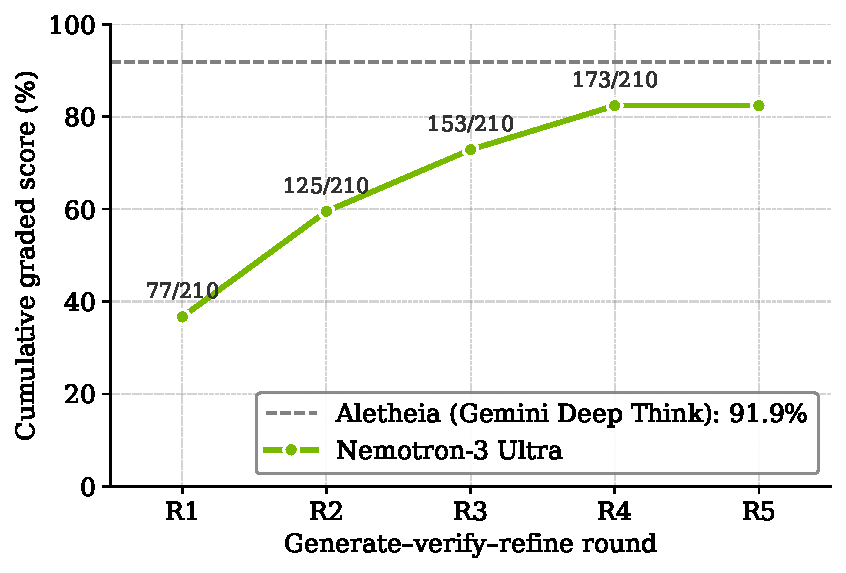
\includegraphics[width=\linewidth]{figures/math_ttc.pdf}
\captionof{figure}{Test-time scaling of \ourmodel on IMO-ProofBench Advanced by round}
\label{fig:math_ttc}
\end{minipage}
\end{figure*}

\subsubsection{Test-time Scaling in Math Olympiad Problems}

\ourmodel achieves strong performance as the underlying model of a high-compute, search-based test-time scaling strategy for Olympiad-level competition mathematics. Following the generate--verify--refine methodology of \citet{shao2025deepseekmath}\footnote{In contrast with the original paper, we started with 128 proof attempts per problem and allowed 512k context length. All other pipeline hyperparameters were identical.} and Nemotron-Cascade-2~\citep{yang2026nemotron}, we evaluate on the IMO-ProofBench Advanced subset \citep{luong2025towards}, IMO 2025, Putnam 2025, and USAMO 2026, with final accuracies reported in Table~\ref{tab:math_ttc}.

Figure~\ref{fig:math_ttc} shows the accuracy of the test-time scaling strategy vs rounds of refinement in the pipeline, as a proxy for compute. The SOTA performance of the Aletheia math research agent \citep{feng2026autonomousmathematicsresearch} is also plotted.

